%%%%%%%%%%%%%%%%%%%%%%%%%%%%%%%%%%%%%%%%%%%%%%%%%%%%
\documentclass[12pt]{report}
\usepackage[a4paper, margin=2cm]{geometry}
\usepackage{graphicx}
\usepackage{url}
\usepackage{tikz}
\usepackage{eso-pic}
\usepackage{booktabs}
\usepackage{longtable}
\usepackage{parskip}
\usepackage{hyperref}
%%%%%%%%%%%%%%%%%%%%%%%%%%%%%%%%%%%%%%%%%%%%%%%%%%%%


%%%%%%%%%%%%%%%%%%%%%%%%%%%%%%%%%%%%%%%%%%%%%%%%%%%%
\newcommand{\papertitle}{The Language Paradox: Investigating the Myth of English-Speaking Employability in Berlin’s Job Market}
\newcommand{\researchquestion}{To what extent does Berlin's reputation as an international, English-friendly city align with the linguistic requirements of its actual job market for non-German speakers?}
\newcommand{\student}{Ali M Abdou, Chakib Khemaissia, Nibras H Nathu, Omid Karimi}
\newcommand{\module}{B124 Academic Writing and Research Methods}
\newcommand{\supervisor}{Vahab Esfandani}
\newcommand{\modleader}{Prof. Dr. Sara Ramzani}
\newcommand{\submissiontime}{SS0325}
%%%%%%%%%%%%%%%%%%%%%%%%%%%%%%%%%%%%%%%%%%%%%%%%%%%%
\renewcommand\maketitle{
	{
		\center
		\begin{tikzpicture}[remember picture, overlay]
			\node[opacity=0.2,inner sep=0pt] at (current page.south) [yshift=5cm]{
				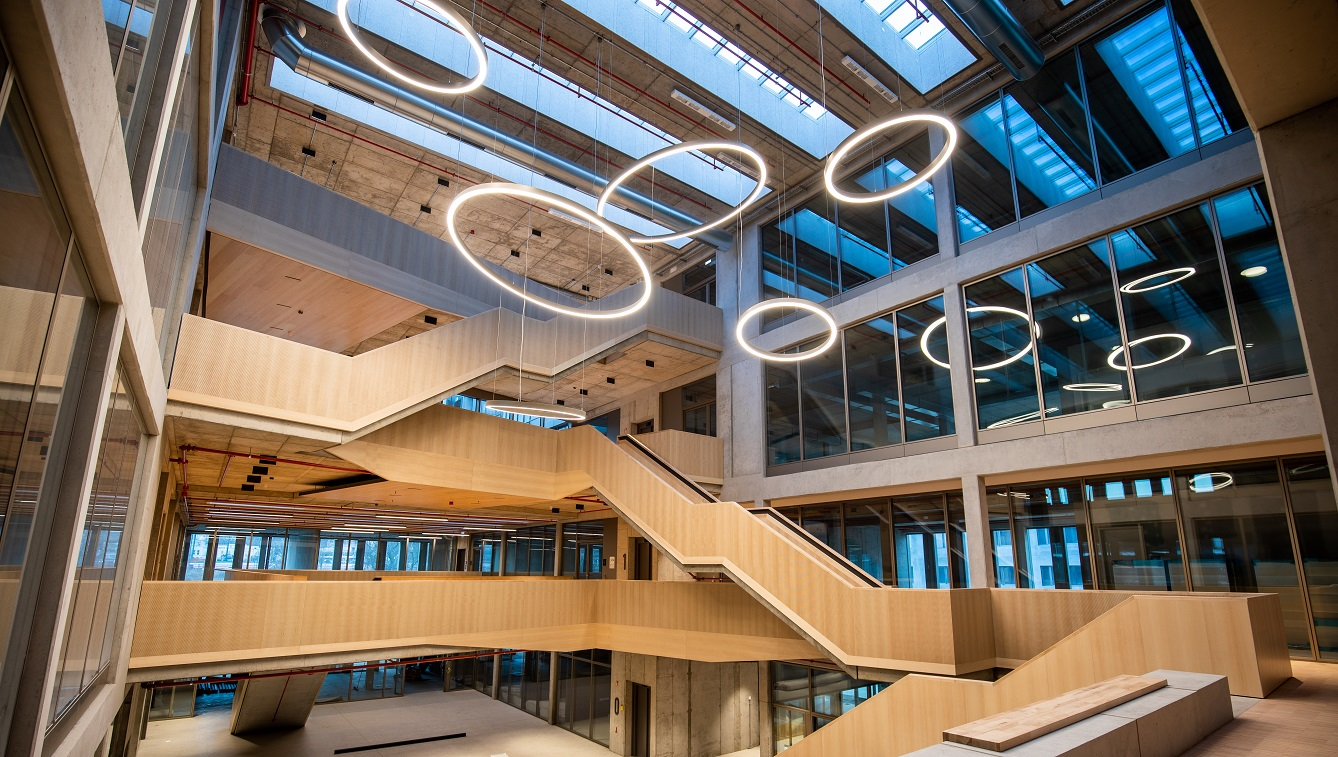
\includegraphics[width=\paperwidth, height=\paperheight, keepaspectratio]{attachments/campus}
			};
		\end{tikzpicture}
		
\includegraphics[width=0.6\textwidth]{attachments/logo}\par
		{\scshape\LARGE\bf Gisma University of Applied Sciences \par}
		\vspace{2cm}
		\rule{\linewidth}{0.5mm}\par
		{\huge\bfseries\papertitle\par}
		\rule{\linewidth}{0.5mm}\par
		\vspace{0.2cm}
		{\Large\student\par}
		\vspace{3.8cm}
		{\large Submitted in  fulfillment of the final assessment for the module\par}
		{\large\bf\module\par}
		\vspace{0.7cm}
		{\large Lecturer\par}
		{\large\bf\supervisor\par}
		\vspace{0.7cm}
		{\large Module Leader\par}
		{\large\bf\modleader\par}
		\vspace{0.72cm}
		{\large\submissiontime\par}
		\thispagestyle{empty} 
		\newpage
	}
}

\newcommand\makesubtitle{
	{
		\center
		
\includegraphics[width=0.4\textwidth]{attachments/logo2}\par
		{\scshape\Large\bf Gisma University of Applied Sciences \par}
		\vspace{0.8cm}
		\raggedright
		\rule{\linewidth}{0.3mm}\par
		\vspace{0.8cm}
		\normalsize
		Paper Title \par
		\textbf{\papertitle}\par
		\vspace{0.8cm}
		Research Question \par
		\textbf{\researchquestion}\par
		\vspace{0.8cm}
		Collaborative report by:  \par
		\begin{tabular}{@{}l@{\hspace{3em}}l@{}}
			\bf\normalsize{Ali Mohamed Abdou} & GH1033452 \\[0.6ex]
			\bf\normalsize{Chakib Khemaissia} & GH1029909 \\[0.6ex]
			\bf\normalsize{Nibras Hassan Nathu} & GH1036309 \\[0.6ex]
			\bf\normalsize{Omid Karimi} & GH1038348 \\[0.6ex]
		\end{tabular}\par
		\vspace{0.8cm}
		{\normalsize Submitted in  fulfillment of the final assessment for the module\par}
		{\normalsize\bf\module\par}
		\vspace{0.7cm}
		{\normalsize Lecturer\par}
		{\normalsize\bf\supervisor\par}
		\vspace{0.7cm}
		{\normalsize Module Leader\par}
		{\normalsize\bf\modleader\par}
		\vspace{0.7cm}
		{\normalsize Submission Quarter\par}
		{\bf\large\submissiontime\par}
		\center
		\thispagestyle{empty}
		\newpage
	}
}

\begin{document} 
%%%%%%%%%%%%%%%%%%%%%%%%%%%%%%%%%%%%%%%%%%%%%%%%%%%%


%%%%%%%%%%%%%%%%%%%%%%%%%%%%%%%%%%%%%%%%%%%%%%%%%%%%
\pagestyle{plain}
\pagenumbering{roman}
\maketitle
\makesubtitle
\chapter*{}
\vspace{17cm}
\hfill\parbox{8cm}{
\raggedleft
	\textit{We confirm that this collaborative report is our own work and that we have documented all sources and materials used.}\par 
	\vspace{1em}
	Berlin, 24 June 2025

	\vspace{3em}
	{\footnotesize Word Count: 3,285}
}
\thispagestyle{empty}
\pdfbookmark[1]{Abstract}{abstract}
\chapter*{Abstract} 
\phantomsection
\noindent\setstretch{1.2}This study examines the disparity between Berlin’s well-established international reputation as an English-friendly city and the actual language requirements that non-German-speaking professionals encounter in the labor market. By employing a mixed-methods approach, the research combines an analysis of current job listings from various industries with primary survey data collected from international students and expatriates residing in the Berlin Metropolitan Area. The findings reveal a significant discrepancy: although the city is perceived as an accessible hub for English speakers, most full-time job listings still require proficiency in German. The survey results reinforce this observation, indicating that many non-German-speaking professionals experience rejection due to insufficient German language skills. At the same time, the perception of an English-only job market is considerably higher than what is observed. The study concludes by emphasizing that having German language skills remains a significant hurdle to employment for non-German speakers in Berlin. It advocates for a more accurate representation of the city’s language job market requirements to help manage expectations and support improved professional integration.
\tableofcontents 
%%%%%%%%%%%%%%%%%%%%%%%%%%%%%%%%%%%%%%%%%%%%%%%%%%%%


%%%%%%%%%%%%%%%%%%%%%%%%%%%%%%%%%%%%%%%%%%%%%%%%%%%%
\clearpage
\pagenumbering{arabic}
\titlespacing*{\chapter}{0pt}{0pt}{0pt}

\chapter{Introduction}

intro \citep{placeholder}

\titlespacing*{\chapter}{0pt}{12pt}{0pt}
\chapter{Foundations}

This is a chapter...
\chapter{Related Work}

This is a chapter...
\chapter{Approach}

This is a chapter...
\chapter{Results and Discussion}
\vspace{5pt}
\section{Job Listing Analysis}
An analysis of 191 Berlin job listings (see \hyperref[appendix:B]{Appendix~B}) revealed that 75.4\% specified listings required at least conversational German (19.9\% conversational, 55.5\% fluent), while 24.6\% required none. Fifty-two percent of listings were posted in English, 47.1\% in German, and 0.5\% in both. This contrasts with national data indicating that 97\% of jobs require German \citep{Jones25}. While the sample shows a greater presence of English, a significant German barrier persists, challenging Berlin’s perceived friendliness to English speakers.

\subsection{Information Technology}
Of 44 IT listings, 34.1\% needed no German, 25\% required conversational German, and 40.9\% needed fluent German. Sixty-five postings were in English. This sector is English-friendly, with many platforms listing English-speaking roles. Many tech companies foster “English-speaking environments,” creating an English-speaking “bubble”.   

\subsection{Finance}
Of 37 finance listings, 62.2\% required fluent German, 13.5\% conversational German, and 24.3\% no German, with 48.6\% being listed in German. This indicates that finance roles, particularly those involving German regulations, often require German fluency.

\subsection{Healthcare}
Core medical professions require German exams (B2-C2). Primary data shows that roles like `Medizinische Fachangestellte' require fluent German. Bureaucratic tasks are primarily in German. This represents a life-critical language barrier. 

\subsection{Education}
The English teaching market is peculiarly saturated. Certified teachers in public schools require proficiency in fluent German. Primary data shows mixed requirements (33.3\% none, 16.7\% conversational, 50\% fluent), with 70.8\% of listings posted in English.

\subsection{Public Services}
Of 24 public service listings, 58.3\% required fluent German, 12.5\% conversational German, and 29.1\% required none, with 50\% listed in English. Public service roles almost universally require proficiency in German due to the state administration and bureaucracy.   

\subsection{Manufacturing}
Of 23 manufacturing listings, 65.2\% required fluent German, 21.7\% required conversational German, and 13\% required no German proficiency. With 39.1\% of being listed in English and 4.3\% being listed in both languages, this suggests that blue-collar work, such as manufacturing, tends to require proficiency in German for ease of communication.

\subsection{Marketing}
Of 29 listings for marketing, 48.3\% required fluent German, 34.5\% required conversational German, and 17.2\% required none. Forty-eight percent of listings were in English. This suggests that German businesses tend to market primarily to German-speaking consumers, rather than international customers, given that the majority of positions require proficiency in the language.

\section{Survey Findings}
\vspace{5pt}
\subsection{Demographics Language Proficiency, and Perceptions of Respondents}
The survey gathered responses from young professionals and students, primarily aged 18-25 (69\%) and 26-35 (23\%). Most respondents held or were pursuing a bachelor’s degree (54\%), while the remainder held or were working towards a master’s degree (46\%). Many respondents were from Gisma University of Applied Sciences, reflecting the demographics of international students and expatriates. A significant majority (69\%) of participants reported Beginner (A1-A2) proficiency in German, with 15\% having no German skills. Additionally, 73\% were fluent in English, while the remaining 27\% possessed intermediate (B1-B2) English skills.

This linguistic profile, which indicates a highly educated group with strong English but limited German, supports the argument that Berlin attracts English-speaking professionals who are underprepared for the broader German-speaking labor market. Respondents indicated that only a tiny number of job listings did not require German language skills. Sixty-two percent reported that only 0-25\% of job listings in their desired field were posted in English, with 19\% reporting 26-60\%. In further support of the assertion that German is almost always required in the workplace, 42\% stated that German was always required in their field, while 38\% said it was often necessary. This inconsistency between Berlin’s English-friendly reputation and its actual job market outlines the widespread reality for job seekers, creating an imminent employment challenge.


\subsection{Impact of German Language Skills on Job Searches}
Sixty-nine percent of participants reported job application rejections due to insufficient German skills. Only 12\% were able to secure employment without fluency in German, primarily in the hospitality and information technology sectors. Additionally, 31\% were not invited to any interviews, suggesting that language barriers hinder initial screening and indicating limited English-only opportunities. This empirical evidence supports the claim that language proficiency has a significant impact on employment.

Before relocating to Berlin, 50\% of participants believed they could find a job there without speaking German, which aligns with the city’s image. However, when asked if Berlin’s English-friendly reputation accurately reflects the job market, 50\% stated that this was not true at all, while an additional 23\% expressed that it was only slightly true. This stark contrast reveals a significant gap between reputation and reality. Berlin’s marketing creates unrealistic expectations that lead to frustration and dissatisfaction for expatriates and international students.

\section{Analysis}
The study reveals a significant gap between Berlin’s image as an English-friendly city and its labor market realities. Survey respondents report a shortage of English-only job listings (0-25\% for 62\%), aligning with national data indicating that 96-97\% of postings require German proficiency. An 88\% rejection rate due to inadequate German skills highlights the linguistic demands in most sectors. The success rate for non-fluent German speakers demonstrates a labor market where English-only positions are rare. While English suffices in tourism, it is insufficient in traditional industries and public services, which are primarily conducted in German. Despite Berlin’s marketing as an English-friendly city, actual labor market conditions require German proficiency, posing challenges for non-German speakers. A lack of German skills hinders career advancement and income growth. Proficiency is crucial for navigating bureaucracy and internal communication. New residency regulations mandating German proficiency formalize this situation, acting as a socio-economic gatekeeper and relegating non-German speakers to a secondary labor market with limited integration opportunities.

Berlin’s competitive market faces an oversaturation of English-only job openings. Recruiters often seek a “perfect fit,” including one that matches their language preferences. Daily life and administrative tasks remain predominantly German-speaking. Implicit German expectations can lead to rejections, and employers may exhibit statistical discrimination. This often limits qualified international professionals to low-skilled roles, leading to underemployment.

The tech and startup ecosystem offers the best path for English-speaking professionals, particularly in software development and AI. Learning German is vital as it broadens job opportunities and enhances career prospects. Government language courses boost employment opportunities. Berlin presents an English-friendly image but reveals a German-dominated reality, requiring job seekers to adapt their strategies accordingly. Opportunities lie in competitive niches, while the broader market remains inaccessible without German. The focus should be on long-term German language investment and targeted networking to break through barriers and achieve integration. \par

\include{chapters/results}
\chapter{Project Closure}

The closure of the project represents the concluding phase of the project lifecycle, encompassing the formal certification of completion, evaluation of outcomes, and verification that deliverables adhere to the mutually agreed-upon standards. Given the intricacy of the CHSR project, the closure process must be executed in a phased and strategic manner to ensure sustainability, compliance, and stakeholder satisfaction.

\section{Closure Criteria}
For each segment, such as the Central Valley IOS, completion is contingent upon the fulfillment of all contractual deliverables (including infrastructure, safety systems, and interoperability), the successful performance testing and commissioning of all systems, and obtaining regulatory approval. A segment shall not be deemed complete unless these three criteria are satisfied. These criteria cannot be prioritized by urgency, as the first pertains to the physical installation of the project, the second concerns safety and operability, and the third involves securing legal approval from state authorities and ensuring compliance with safety, environmental, and technical standards. \par

\section{Acceptance Process}
The acceptance process begins with the Project Management Office issuing formal handover reports to the CHSR authority’s executive board and operations division, indicating that the project is ready for operational review. At the same time, an Operational Readiness Review is conducted to carefully verify that all key components, including sufficient staffing, robust systems, and detailed maintenance plans, are in place and prepared for deployment. The final crucial step is obtaining stakeholder sign-off, which involves securing approval from key stakeholders, including the State of California, the Federal Railroad Administration, and relevant community representatives, especially those in areas heavily affected by eminent domain or construction activities. This process ensures that all concerns are adequately addressed before the project is officially accepted.

\section{Documentation and Archiving}
Any project requires thorough documentation for future research and growth. Fortunately, the CHSR authority is mandated by the State of California’s Legislative Analyst’s Office to submit annual project update reports and business plan updates every 2-4 years (or whenever there is a change to the plan). This requirement will simplify archiving, as by the project’s end, only minor edits will be needed for the latest business plan and project update report to accurately reflect the project’s overall progress. This includes final risk registers, procurement logs, financial records, commissioning records, warranties, legal documents, and stakeholder agreements. Additionally, all documentation must be stored in a centralized digital repository to comply with California’s Public Records Act (California Government Code, § 6250 et seq.).

\section{Conclusions and Transitions}
Project reviews shall be conducted to assess schedule compliance, cost deviations, the efficacy of stakeholder engagement strategies, contractor and supplier performance, and the effectiveness of risk management. These insights shall offer a prospective outlook for CHSR segments and other significant infrastructure endeavors within California. Upon completion, responsibilities will be transferred from the Project Management Office to the Operations and Maintenance Division, which will oversee the daily service operations, ongoing maintenance, and user feedback collection of the CHSR. Staff recruitment, training, and onboarding procedures should commence approximately six months prior to the project’s completion to facilitate a seamless transition. \par
\clearpage
%%%%%%%%%%%%%%%%%%%%%%%%%%%%%%%%%%%%%%%%%%%%%%%%%%%%


%%%%%%%%%%%%%%%%%%%%%%%%%%%%%%%%%%%%%%%%%%%%%%%%%%%%
\bibliographystyle{apalike}
\renewcommand{\bibname}{References}
\bibliography{attachments/bibliography}
%%%%%%%%%%%%%%%%%%%%%%%%%%%%%%%%%%%%%%%%%%%%%%%%%%%%


%%%%%%%%%%%%%%%%%%%%%%%%%%%%%%%%%%%%%%%%%%%%%%%%%%%%
\end{document}
%%%%%%%%%%%%%%%%%%%%%%%%%%%%%%%%%%%%%%%%%%%%%%%%%%%%